\documentclass[sigconf,anonymous,review]{acmart}

\AtBeginDocument{%
  \providecommand\BibTeX{{Bib\TeX}}}

% Anonymous review draft. Camera-ready metadata will be supplied by ACM.
\setcopyright{none}
\settopmatter{printacmref=true}
\renewcommand\footnotetextcopyrightpermission[1]{}
\acmConference[WWW '27]{The ACM Web Conference 2027}{May 10--14, 2027}
  {Dublin, Ireland}

\begin{document}

\title{HyRex: Cost-Aware Prefix Recovery for Hybrid LLM Serving}

\author{Anonymous Author(s)}

\begin{abstract}
Multi-turn conversations and Web agents repeatedly invoke a large language
model (LLM) with a growing history, making prefix-cache recovery critical to
time to first token (TTFT).  Existing cache systems work well for Transformer
models, whose reusable history is represented by a homogeneous key-value (KV)
cache.  Hybrid LLMs, however, interleave full-attention layers with recurrent
layers and therefore maintain two heterogeneous histories: fine-grained KV
pages and coarse recurrent-state checkpoints.  Treating both histories as one
prefix length either discards reusable KV pages or requires dense, expensive
state checkpoints.

We characterize this problem on Qwen3.5-9B with real multi-turn conversations.
Coarse state alignment replays 391--400 tokens per resumed request on average.
Independent matching increases reusable full-attention KV by 29.4\%, yet does
not improve TTFT because the missing recurrent state still requires most of
the suffix forward pass.  Adding one exact tail-state checkpoint reduces
full-model replay by 59.3--63.3\%, but is not uniformly beneficial.  In a
controlled gap sweep, exact steady-state recovery is 4.1--10.2\% slower than a
matched aligned path when it avoids at most 384 replay tokens, yet becomes
16.3\% faster when it avoids 512.  These results expose a missing abstraction:
a cache hit is not a scalar prefix length, and the deepest hit is not
necessarily the fastest recovery path.

We present \emph{HyRex}, a cost-aware recovery framework that represents a
hybrid prefix as independently matched KV and recurrent-state boundaries.
HyRex places a small number of high-value state checkpoints, constructs exact
recovery paths over heterogeneous cached states, and selects a path according
to its predicted compute, transfer, and batching cost.  Its central goal is
not to maximize cache-hit length, but to minimize end-to-end recovery latency
while preserving exact model semantics and efficient batched execution.
% TODO: Add final end-to-end HyRex speedup and capacity results after the
% online path selector and batch-preserving checkpoint path are evaluated.
\end{abstract}

\ccsdesc[500]{Computer systems organization~Cloud computing}
\ccsdesc[500]{Computing methodologies~Natural language processing}
\ccsdesc[300]{Information systems~Web applications}

\keywords{large language model serving, hybrid LLM, prefix caching,
recurrent state, KV cache, multi-turn conversation, Web agents}

\maketitle

\section{Introduction}

Large language model services are evolving from one-shot question answering
to stateful Web applications, including multi-turn assistants, coding agents,
and tool-using agents.  A request in these applications typically contains the
entire previous interaction and appends only a short user message, tool result,
or model observation.  Recomputing the shared history in every turn wastes GPU
cycles and directly increases time to first token (TTFT), the latency most
visible to an interactive user.  Prefix caching avoids this work by retaining
the model state of previous requests and reusing the longest matching prefix.
Systems such as vLLM, SGLang, and LMCache further page, share, and offload these
caches across requests and memory tiers~\cite{kwon2023vllm,zheng2024sglang,cheng2025lmcache}.

This seemingly simple abstraction is challenged by the growing adoption of
\emph{hybrid} LLMs.  Unlike a Transformer, a hybrid model interleaves
full-attention layers with recurrent layers such as state-space or gated
linear-attention layers~\cite{gu2024mamba,pan2025marconi}.  A full-attention
layer stores one KV entry per token and naturally supports fine-grained paging.
A recurrent layer instead compresses its entire history into a fixed-size
state that is updated in place.  Reusing a recurrent prefix therefore requires
an exact state checkpoint at a valid historical boundary.  The two state types
differ in size, update semantics, and natural caching granularity.

Current serving stacks nevertheless expose cache reuse as a single scalar
prefix length.  Let $L_{KV}$ denote the deepest contiguous full-attention KV
hit and $L_S$ the position of the deepest available recurrent-state checkpoint.
When $L_{KV} > L_S$, a conservative recovery path reports
$\min(L_{KV},L_S)$ as the reusable prefix.  For example, Qwen3.5-9B may retain
KV pages through token 1,584 while its latest recurrent checkpoint is at token
1,056.  Falling back to token 1,056 leaves 528 tokens of valid KV underused.
This mismatch occurs repeatedly in append-heavy conversations because the KV
page size is much smaller than the recurrent checkpoint interval.

\begin{figure*}[t]
  \centering
  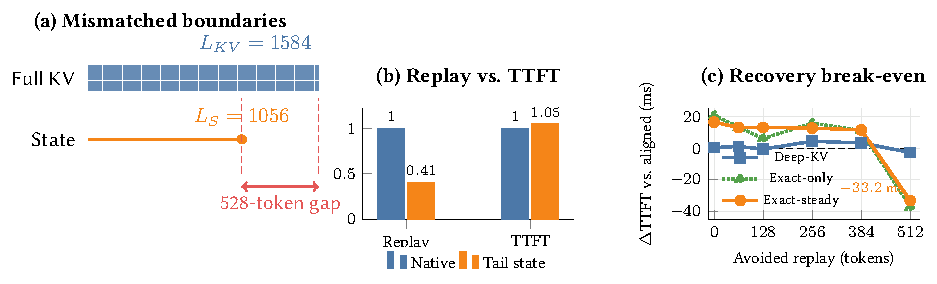
\includegraphics[width=\textwidth]{figures/motivation.pdf}
  \caption{Motivating hybrid-recovery results on Qwen3.5-9B.  (a) Fine-grained
  Full-KV pages can extend beyond the latest recurrent checkpoint.  (b) Across
  16 real sessions at concurrency one, one exact tail state reduces mean replay
  from 391.5 to 159.2 tokens (59.3\%) but increases mean TTFT from 159.38 to
  167.84~ms (5.3\%).  Values are normalized to native recovery.  (c) A
  controlled sweep reports median TTFT relative to a matched aligned path.
  Deep-KV recovery has no systematic gain; exact recovery pays a fixed cost at
  small gaps but saves 33.2~ms in steady state when it avoids 512 replay tokens.
  These are characterization results, not the final HyRex performance.}
  \Description{Three panels show mismatched KV and recurrent-state boundaries,
  normalized replay and TTFT bars for native and tail-state recovery, and
  controlled TTFT deltas as the avoided replay gap increases.}
  \label{fig:motivation}
\end{figure*}

One might fix the mismatch by indexing the two states independently: restore
the checkpoint at $L_S$, load KV through $L_{KV}$, and replay only the missing
recurrent history.  Our measurements show that this intuitive solution is
insufficient.  Across four real ten-turn conversations, independent matching
increases reusable full-attention KV from 32,736 to 42,368 tokens, or 29.4\%.
Yet it yields no TTFT gain and is 1.3\% slower in the measured run.  Profiling
explains why.  Hybrid layers are interleaved, so
advancing recurrent state still requires the suffix activations produced by
attention and MLP layers.  Deeper KV avoids K/V projection for only eight of
the model's 32 layers; it does not skip the full suffix forward pass.  Smaller
split GEMMs and additional launches can erase even that narrow saving.

The opposite solution is to store recurrent state close to every reusable KV
boundary.  It reduces the complete suffix forward pass, but moves the cost to
checkpoint creation, transfer, and capacity.  In Qwen3.5-9B, one padded
recurrent checkpoint occupies 49.5~MiB.  Our ABBA experiment shows that one
replaceable tail checkpoint reduces full-model replay from 400.0 to 132.5
tokens per continuation (63.3\%), while an unconditional implementation raises
mean TTFT from 152.37 to 170.10~ms.  A controlled sweep makes the break-even
explicit.  Relative to an implementation-matched aligned path, exact
steady-state recovery is 4.1--10.2\% slower when it avoids 0--384 replay
tokens, but 16.3\% faster when it avoids 512.  At that point, checkpoint
maintenance costs 3.9~ms in median TTFT relative to recovery alone, but the
path remains 33.2~ms faster than alignment.  Thus, neither maximum cache depth
nor minimum recomputation is a reliable recovery objective.

Concurrency makes the tradeoff sharper.  On 16 real sessions, a tail
checkpoint consistently removes about 60\% of replayed tokens.  Nevertheless,
its TTFT overhead grows from 5.3\% at concurrency one to 24.0\% at concurrency
16.  The main cause in our current prototype is not the lookup itself: exact
checkpoint capture slices a packed prefill into request-local recurrent calls,
thereby losing the batching efficiency of the native path.  This observation
rules out a per-request optimization that appears attractive in isolation.
Hybrid recovery must preserve batching and account for shared runtime
resources.

These observations expose two coupled challenges.

\textbf{C1: Constructing and selecting executable heterogeneous recovery
paths.}  A system cannot equate a deeper KV match with a deeper executable
prefix.  It must compose KV pages and recurrent checkpoints without violating
layer dependencies, then choose among aligned replay, deep-KV replay, and exact
state recovery.  Their costs vary with replay shape, transfer layout, batch
size, and contention; a path that saves arithmetic can still lose to the
native fast path.

\textbf{C2: Recovery-aware state materialization and cache orchestration.}
Dense recurrent checkpoints eliminate replay but impose prohibitive capture,
capacity, and transfer costs; sparse checkpoints leave variable replay gaps.
Useful positions depend on future session reuse, turn and branch boundaries,
and whether concurrent requests can share packed execution.  The system must
jointly decide which states to create, retain, transfer, and batch under finite
CPU-cache and PCIe budgets.

We present \emph{HyRex}, a cost-aware heterogeneous prefix-recovery system.
HyRex replaces the scalar cache-hit abstraction with a state vector
$\mathcal{H}=(L_{KV},L_S)$ and independently indexes full-attention pages and
recurrent checkpoints.  Given a resumed request, it constructs multiple exact
recovery paths and estimates their end-to-end cost instead of blindly choosing
the deepest hit.  HyRex complements this runtime decision with sparse,
workload-aware checkpoint placement: it prioritizes high-value locations such
as conversation tails, frequently reused boundaries, and agent branch points.
Finally, its execution path coalesces fine-grained matches into coarse data
movement and preserves packed recurrent execution across concurrent requests.

This paper makes the following contributions:

\begin{itemize}
  \item We identify and characterize \emph{mismatched heterogeneous recovery
  boundaries} in hybrid LLM serving.  Our experiments show that deeper cache hits
  and fewer replayed tokens do not necessarily reduce TTFT.

  \item We introduce a decoupled representation and exact recovery mechanism
  for independently matched full-attention KV and recurrent states, turning
  hybrid recovery into an explicit path-selection problem.

  \item We design cost-aware checkpoint placement and recovery selection that
  jointly consider replay compute, cache capacity, transfer organization, and
  batch efficiency.

  \item We implement HyRex on vLLM and LMCache and evaluate it with real
  multi-turn conversation and agent workloads across cache budgets and
  concurrency levels.
  % TODO: Add the final headline evaluation result here.
\end{itemize}

\section{Background and Motivation}
\label{sec:motivation}

\subsection{Prefix Recovery in Hybrid LLMs}

Paged prefix caching divides a Transformer's KV cache into independently
managed token blocks~\cite{kwon2023vllm}.  A cached block is reusable whenever
its token prefix and model configuration match, so a request can resume after
the deepest contiguous hit.  CPU-offload systems extend this mechanism beyond
GPU capacity by retrieving evicted blocks before prefill~\cite{cheng2025lmcache}.

Hybrid models add recurrent state to this path.  Suppose KV pages are available
through $L_{KV}$ and a recurrent checkpoint $S_{L_S}$ summarizes tokens
$[0,L_S)$.  Exact decoding at position $L$ requires both valid KV for all
full-attention layers and recurrent state $S_L$ for every recurrent layer.  If
$L_S < L_{KV}$, using $S_{L_S}$ directly at $L_{KV}$ is incorrect.  The system
must either (i) resume all layers at $L_S$, (ii) replay $[L_S,L_{KV})$ while
protecting loaded KV, or (iii) load another exact state closer to $L_{KV}$.
These are semantically equivalent only when their state ownership and execution
dependencies are handled correctly; their latency costs can differ widely.

Marconi recognizes that recurrent states make hybrid prefix entries large and
uses reuse- and FLOP-aware admission and eviction~\cite{pan2025marconi}.  HyRex
is complementary: it focuses on what happens \emph{after} heterogeneous cached
objects have been found, including how to compose them and which correct
recovery path minimizes TTFT under CPU offload.

\subsection{Characterization Methodology}

We use Qwen3.5-9B in BF16 eager mode with vLLM and an LMCache CPU tier.  The
model contains 32 layers, including eight full-attention layers and 24 recurrent
layers.  Full-attention KV is matched in 16-token pages, whereas the native
hybrid execution contract exposes recurrent checkpoints at 528-token
boundaries.  Native recovery uses the connector-required 528-token prefill
budget.  To isolate recovery-boundary effects from implementation differences,
we additionally compare aligned, deep-KV, and exact-state paths built on the
same single-forward implementation with a 2,112-token budget.  Unless stated
otherwise, every measured request generates one token; we clear the GPU prefix
cache after each request while retaining the CPU cache, forcing the next turn
to exercise CPU recovery.  All paths use the same LMCache IPC transport.

Our workloads contain real cumulative ShareGPT conversations.  The small ABBA
study uses four sessions with ten turns each.  The larger screening study uses
16 sessions, 120 requests, and 104 continuation requests.  All services receive
unrelated warmup requests before measurement.  We report first-turn requests
separately because they have no reusable session prefix.  Finally, a controlled
sweep fixes the recurrent boundary at 1,056, appends 128 new tokens, and places
the previous turn 0--512 tokens beyond that boundary.  Each point contains five
repetitions with a verified GPU-cache reset; Figure~\ref{fig:motivation}(c)
reports medians to resist isolated host-runtime outliers.

\begin{table}[t]
  \caption{Characterization of native aligned recovery and an exact
  replaceable tail checkpoint on 16 real sessions.  TTFT includes queueing.}
  \label{tab:motivation}
  \centering
  \small
  \begin{tabular}{lrrr}
    \toprule
    & Native & Tail state & Change \\
    \midrule
    Mean replay (tokens), C=1 & 391.5 & 159.2 & $-59.3\%$ \\
    Mean TTFT (ms), C=1       & 159.38 & 167.84 & $+5.3\%$ \\
    P95 TTFT (ms), C=1        & 216.74 & 189.45 & $-12.6\%$ \\
    Mean TTFT (ms), C=4       & 323.07 & 358.27 & $+10.9\%$ \\
    Mean TTFT (ms), C=8       & 472.41 & 576.26 & $+22.0\%$ \\
    Mean TTFT (ms), C=16      & 738.42 & 915.89 & $+24.0\%$ \\
    \bottomrule
  \end{tabular}
\end{table}

\subsection{Finding 1: A Deeper KV Hit Is Not a Deeper Executable Prefix}

Independent KV/state matching recovers 9,632 additional KV-token positions
across the four-session workload.  However, a representative request with
$L_S=528$, $L_{KV}=752$, and length 831 still executes 303 tokens through the
model.  Reusing the middle 224 KV entries removes only their K/V projections.
The profiled full-attention projection time changes from 1.626~ms with fused
QKV to 1.741~ms with split Q and new-KV projections; total GPU-kernel time is
47.224 versus 47.405~ms.  Fine-grained reuse therefore exposes a composition
problem, not an automatic full-forward saving.  The controlled sweep confirms
this result: Deep-KV reports progressively deeper hits, from 1,056 to 1,568
tokens, but its median TTFT stays within $-2.7$ to $+4.4$~ms of the matched
aligned path because complete-model replay still begins at the same recurrent
checkpoint.

\subsection{Finding 2: Exact Tail States Have a Request-Dependent Break-even}

A state checkpoint at the deepest complete KV boundary allows all layers to
resume after that boundary.  It removes 267.6 replayed tokens per continuation
on average in the ABBA experiment, but one such checkpoint occupies 49.5~MiB
in the current padded LMCache transport layout, and its unconditional path is
11.6\% slower.  The sign changes with the avoided
work.  In the controlled sweep, the matched aligned path executes
$128+g$ tokens for gap $g$, while exact recovery always executes 128.  Exact
steady-state recovery remains 11.6--16.6~ms slower in median TTFT for
$g\le384$, but becomes 33.2~ms faster at $g=512$ (166.35 versus 199.57~ms).
Recovery without creating the next checkpoint reaches 162.43~ms at that point,
quantifying a 3.92~ms median maintenance cost.  Across the 16-session workload,
tail recovery similarly becomes attractive primarily for large gaps.  This
request-dependent break-even motivates a measured end-to-end cost model rather
than one global token threshold.

\subsection{Finding 3: Recovery Must Preserve Batching}

Table~\ref{tab:motivation} shows that the same tail policy deteriorates as
concurrency increases even though its replay reduction remains about 60\%.
Tracing attributes the trend to request-local checkpoint execution: the
prototype slices each request from the packed prefill, invokes recurrent
segments separately, clones each state, and concatenates outputs.  Native
execution instead processes the packed recurrent batch together.  This result
motivates batch-preserving checkpoint kernels and a scheduler that can disable
an otherwise useful recovery path when its batching loss exceeds saved compute.

\section{HyRex Overview}
\label{sec:overview}

HyRex treats recovery as a shortest-path problem over exact cached states.  A
request first performs independent lookup and obtains its KV and recurrent
boundaries.  The recovery planner then considers three basic paths: aligned
coarse recovery, deep-KV recovery with recurrent replay, and exact recovery from
a selected sparse state checkpoint.  A lightweight cost model predicts each
path's replay, H2D transfer, checkpoint, and batching cost and selects the
lowest-latency valid path.

The checkpoint manager maintains native coarse states and a small budget of
additional exact states.  Candidate states arise at complete KV boundaries,
with priority given to turn ends and repeatedly reused agent boundaries.  The
manager admits a candidate only when its expected future replay saving exceeds
its capture, transfer, and capacity cost.  Fine-grained keys remain useful for
matching, but HyRex coalesces consecutive KV pages and state objects for data
movement.  Across concurrent requests, it groups equal recovery segments into
packed recurrent calls rather than serializing requests.  The following
sections detail the index, placement policy, path cost model, and
batch-preserving execution engine.

\bibliographystyle{ACM-Reference-Format}
\bibliography{references}

\end{document}
